\chapter{Fundamental Building Blocks}
Embedded software must run at a required rate to meet system deadlines, must meet power consumption
requirements, must meet timing requirements and must fit into the allowed amount of memory.


Given these constraints, everything is mostly done from scratch and it's hard to find perfect libraries for
our applications.


Despite this, there are basic building blocks that can compose a program.

\section{Finite State Machines - FSMs}

An FSM is simply a machine that reacts to inputs via states.

\begin{figure}[H]
    \centering
    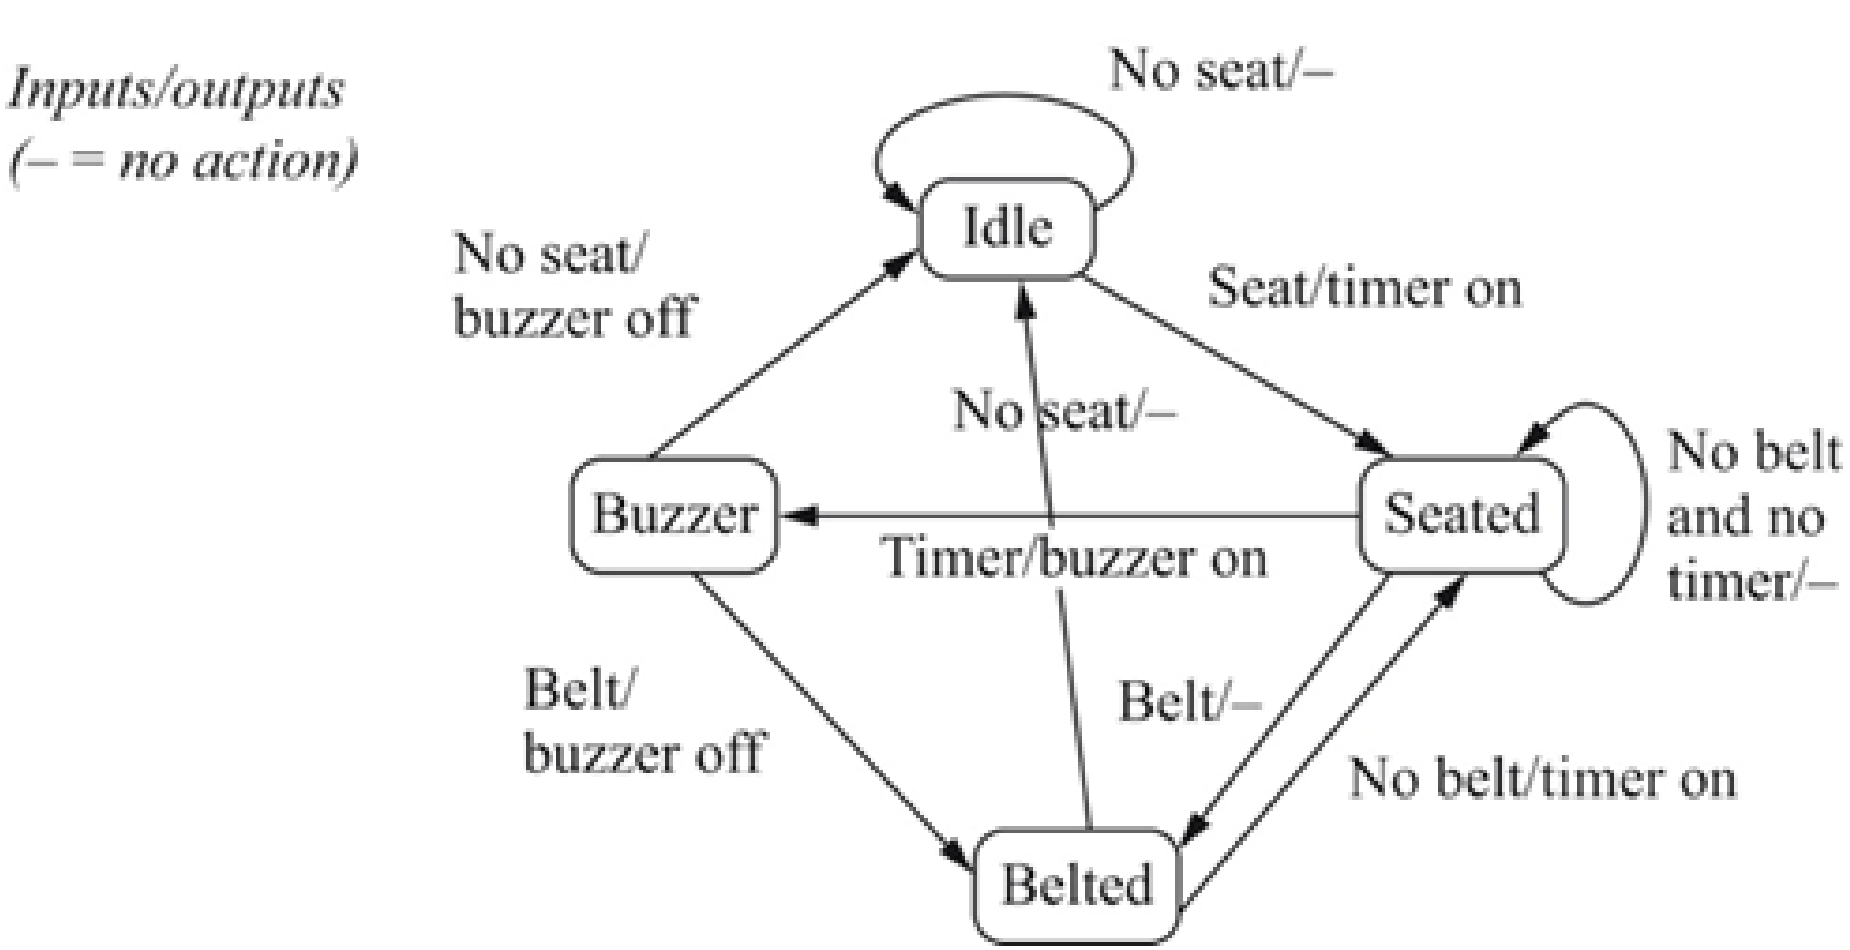
\includegraphics[width=0.5\linewidth]{img/image_60.png}
    \caption{Simple example of FSM}
\end{figure}

We can model it using this Pseudo-Code:


\begin{lstlisting}[language=c++]

    #define IDLE 0
    #define SEATED 1
    #define BELTED 2
    #define BUZZER 3
    
    switch(state) { /* check the current state */
    
        case IDLE:
             if (seat){ state = SEATED; timer_on = TRUE; }
             /* default case is self-loop */
             break;
        case SEATED:
             if (belt) state = BELTED; /* won't hear the buzzer */
             else if (timer) state = BUZZER; /* did not put on belt in time */
             /* default case is self-loop */
             break;
        case BELTED:
             if (!seat) state = IDLE; /* person left */
             else if (!belt) state = SEATED; /* person still in seat */
             break;
        case BUZZER:
             if (belt) state = BELTED; /* belt is on---turn off buzzer */
             else if (!seat) state = IDLE; /* no one in seat-turn off buzzer */
             break;
    }
\end{lstlisting}


\paragraph{NOTE:} Using function pointers decreases the complexity of the FSM program.


\begin{figure}[H]
    \centering
    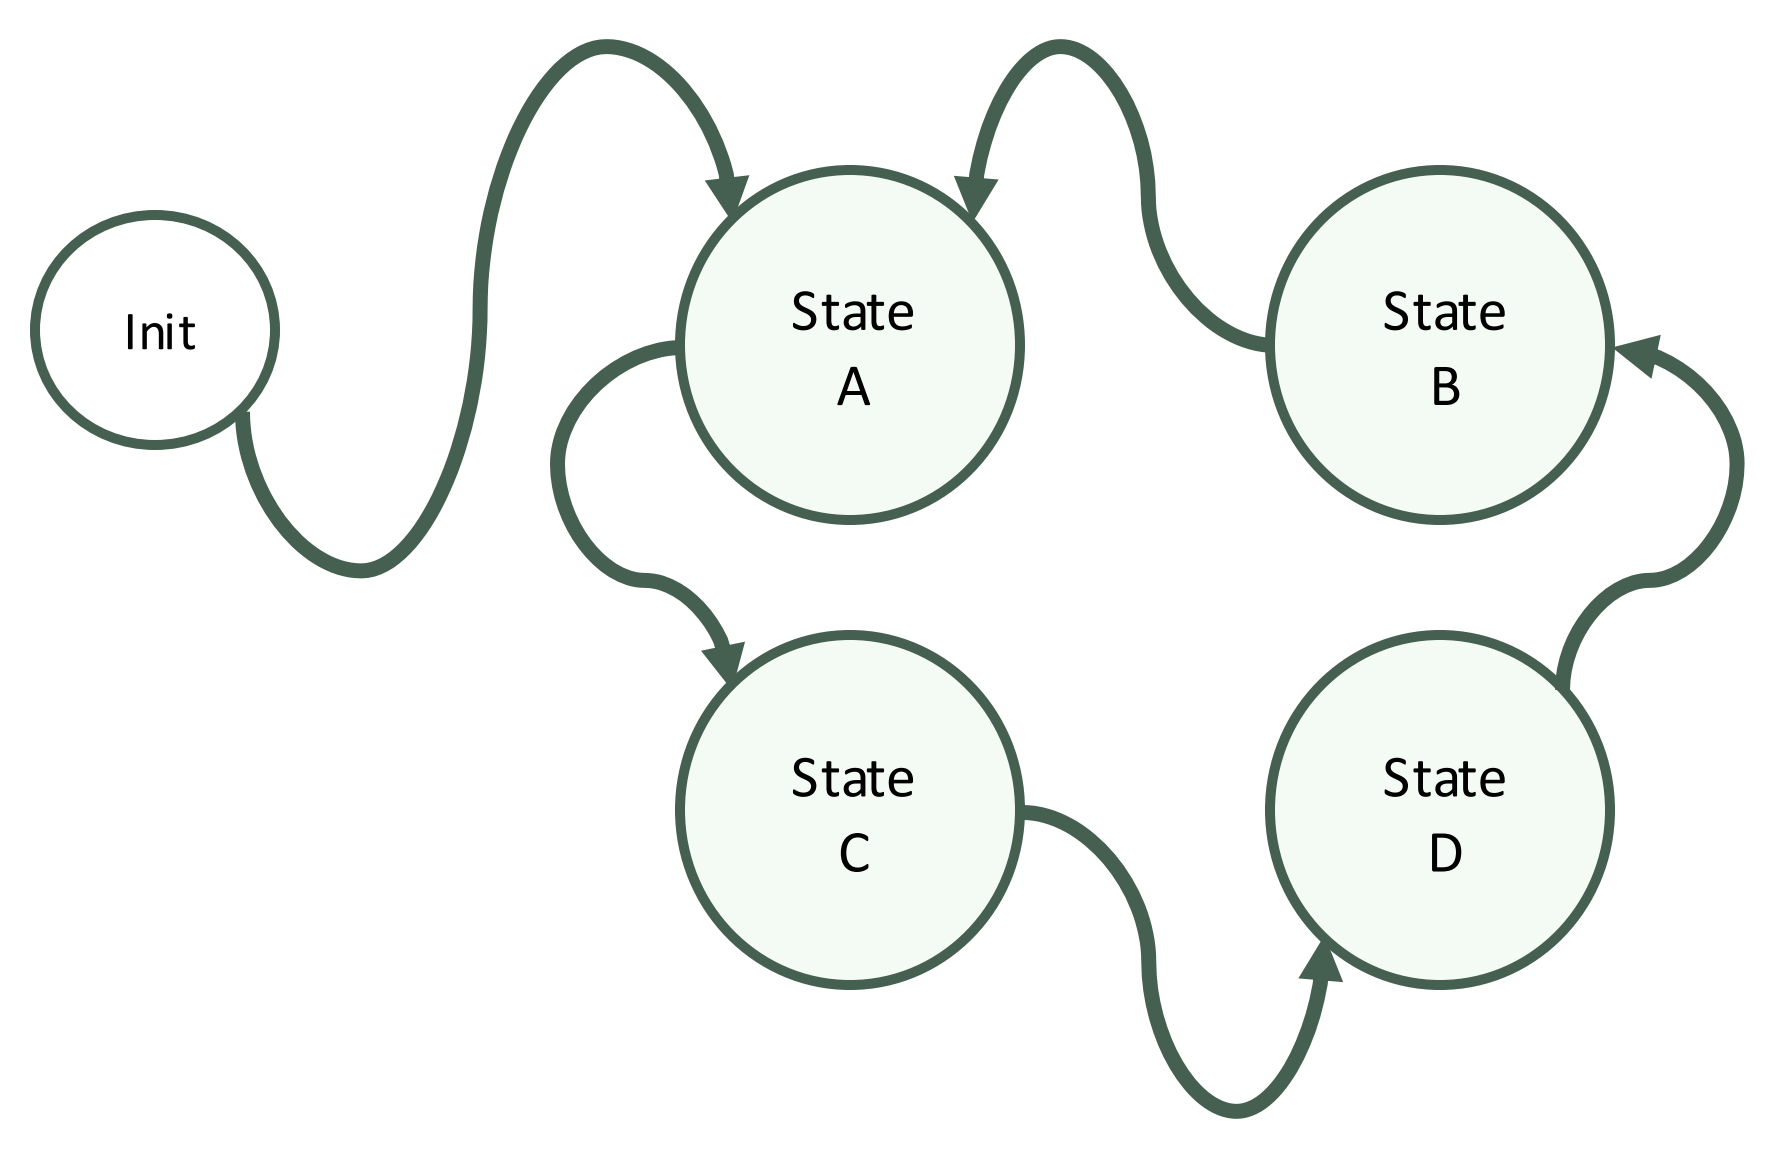
\includegraphics[width=0.6\linewidth]{img/image_61.png}
\end{figure}

\subsection{Define states and and state machine structure:}
\begin{lstlisting}[language=c++]

    typedef enum{
        STATE_A;
        STATE_B;
        STATE_C;
        STATE_D;
        NUM_STATES
    }State_t;
    
    typedef struct{
        State_t state; /* defines the command */
        void (*func)(void); /* defines the function to execute */
    } StateMachine_t;
\end{lstlisting}



\subsection{Declare functions that implement states, variable to hold current state and the state machine itself:}

\begin{lstlisting}[language=c++]

    /* state machine function prototypes */
    void fn_StateA(void);
    void fn_StateB(void);
    void fn_StateC(void);
    void fn_StateD(void);
    
    /* variable that holds the current state */
    State_t cur_state = STATE_A:
    
    StateMachine_t StateMachine[] = {
        {STATE_A, fn_StateA},
        {STATE_B, fn_StateB},
        {STATE_C, fn_StateC},
        {STATE_D, fn_StateD}
    } ;
\end{lstlisting}

\newpage

\subsection{Fill the functions:}

\begin{lstlisting}[language=c++]

    void fn_StateA(void){
        /* add the necessary code here */
        cur_state = STATE_B;
    }
    void fn_StateB(void){
        /* add the necessary code here */
        cur_state = STATE_C;
    }
    void fn_StateC(void){
        /* add the necessary code here */
        cur_state = STATE_D;
    }
    void fn_StateD(void){
        /* add the necessary code here */
        cur_state = STATE_A;
    }
\end{lstlisting}



\subsection{Run function:}
\begin{lstlisting}[language=c++]

    void run(void){    
        if(cur_state < NUM_STATES){
            (*StateMachine[cur_state].func)();
        }else{
            // error
        }
    }
\end{lstlisting}

\section{Circular Buffer}

Circular buffers are a data structure useful for stream-oriented processing (where data comes regularly
and must be processed on the fly, basically we can read values but also must consume values).

\section{Queue}

Queues are a data structure useful for data that arrives and departs at unpredictable times.
A synonym of queue is \textbf{elastic buffer.}
\paragraph{}
One way to implement a queue is through linked lists, that allows the queue to grow to an arbitrary size at
the cost of overhead of dynamic memory allocation (therefore not recommended).
Another way is through an array to hold all the data.
\paragraph{}
A queue may have varying numbers of elements in it as it doesn't have to accommodate all of the incoming
data, but a circular buffer will always have a fixed number of data.


\section{Producer/Consumer problems}

Some aspects of an application can be a producer and others can be a consumer. This is meant in
regards to writing (producing) and reading (consuming) data. Basically we should strive to keep the loads
balanced

\section{Pragma}

A \verb|pragma| is a compiler directive, usually platform-specific.

\begin{figure}[H]
    \centering
    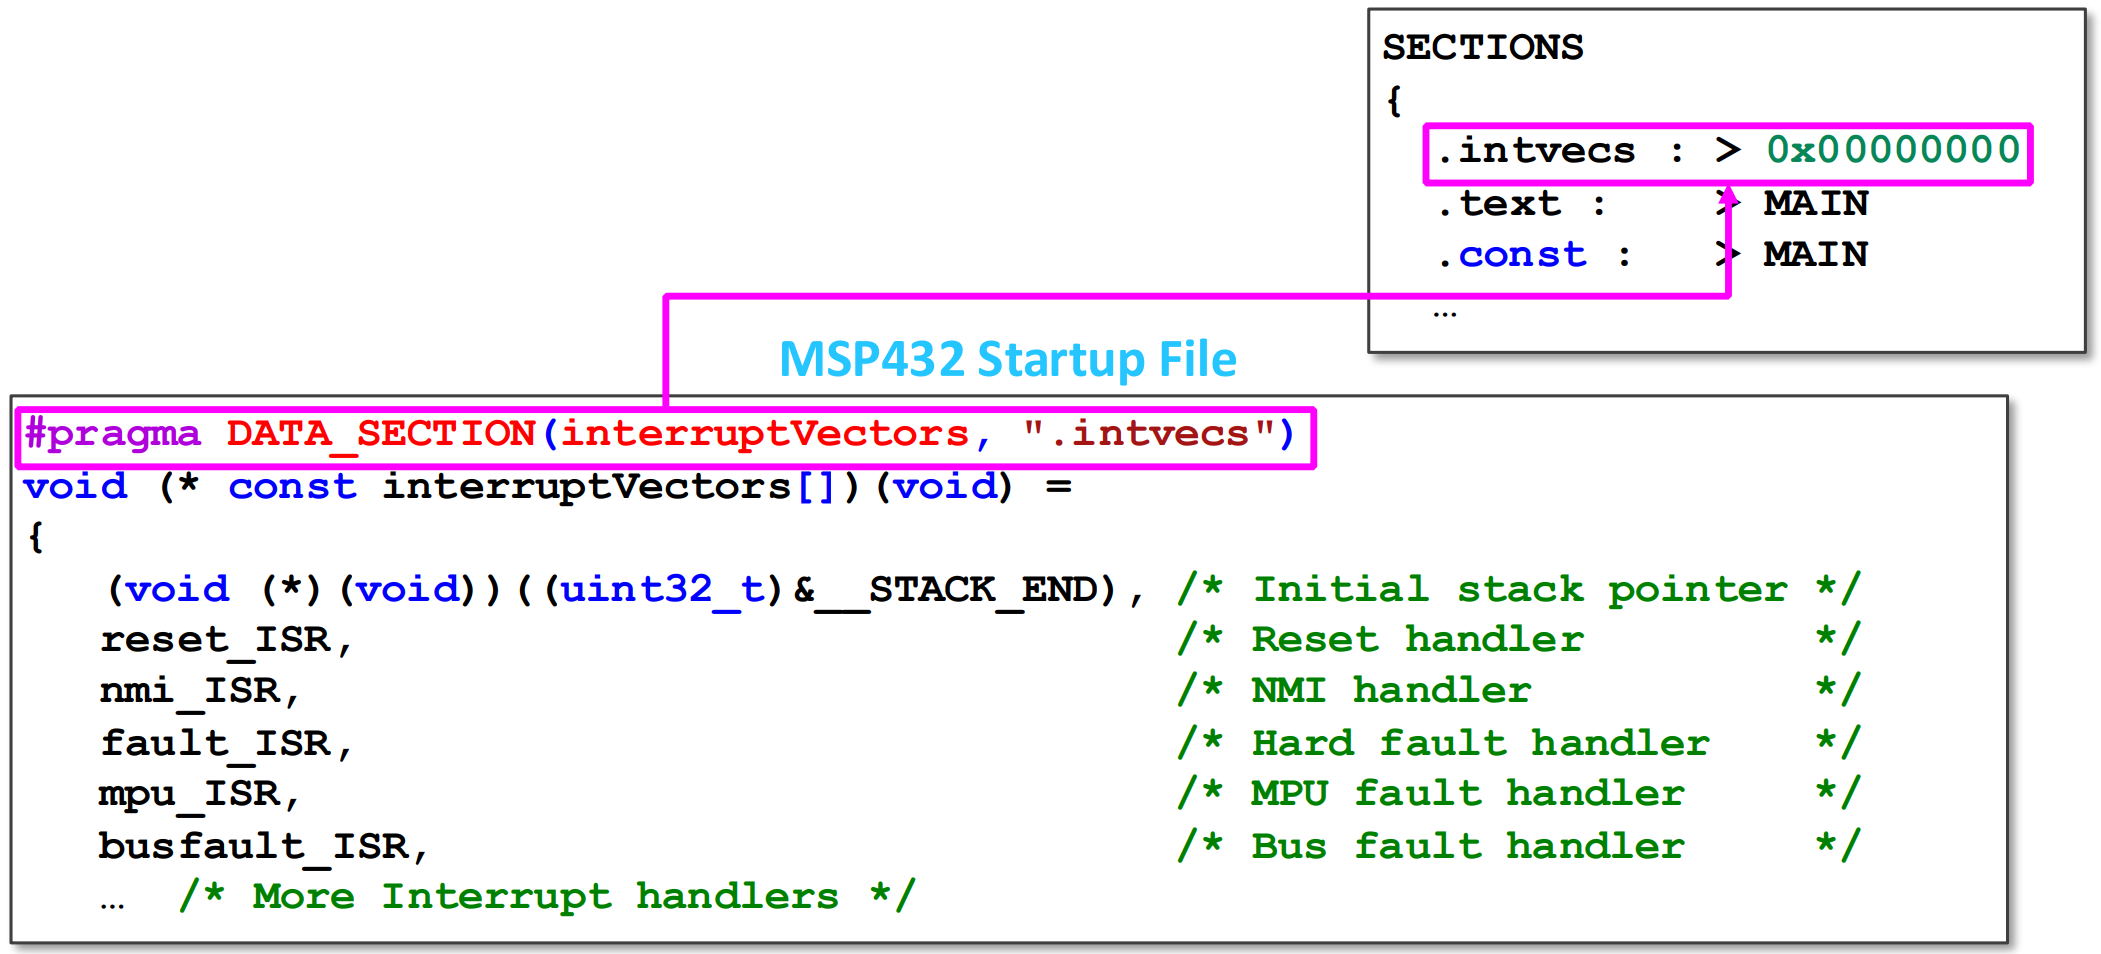
\includegraphics[width=0.75\linewidth]{img/image_62.png}
\end{figure}
In this case, it is used to specify the data section of interruptVectors in .intvects
interruptVectors is the Interrupt Vector Table.

\paragraph{}
Since it is a constant array it will be placed in the Flash memory.
The first entry is the Initial Stack Pointer to initialised the Core CPU registers.

The other five entries are High-Priority ARM Core Exceptions.
The rest of the handlers are for GPIO interrupts


\section{Default Handler}

\begin{lstlisting}[language=c++]

    ...
    /* Forward declaration of the default fault handlers. */
    void Default_Handler (void) __attribute__((weak));
    ...
    /* This is the code that gets called when the processor receives an unexpected */
    /* interrupt. This simply enters an infinite loop, preserving the system state */
    /* for examination by a debugger. */
    
    void Default_Handler(void){
    
        /* Fault trap exempt from ULP advisor */
        #pragma diag_push
        #pragma CHECK_ULP("-2.1")
        
        /* Enter an infinite loop. */
        while(1){
        
        }
        
        #pragma diag_pop
    }
\end{lstlisting}


\verb|__attribute__((weak))| means that it can be overridden by the developer

\subsection{Overriding Default Handlers}

\begin{lstlisting}[language=c++]

    ...
    extern void PORT1_IRQHandler (void) __attribute__((weak,alias("Default_Handler")));
    extern void PORT2_IRQHandler (void) __attribute__((weak,alias("Default_Handler")));
    extern void PORT3_IRQHandler (void) __attribute__((weak,alias("Default_Handler")));
    extern void PORT4_IRQHandler (void) __attribute__((weak,alias("Default_Handler")));
    extern void PORT5_IRQHandler (void) __attribute__((weak,alias("Default_Handler")));
    extern void PORT6_IRQHandler (void) __attribute__((weak,alias("Default_Handler")));
    ...
\end{lstlisting}

\textit{alias} means that it defaults to \verb|Default_Handler| if it is not implemented.
\textit{extern} means that the function can be defined in other source files.


\section{Implementing Interrupts}

We can do this by using Interrupt \textbf{Edge Select Registers} (PxIES), \textbf{Interrupt Flag Registers} (PxIFG),
and \textbf{Interrupt Enable Registers} (PxIE).

\paragraph{Example: } left button P1.1
\begin{lstlisting}[language=c++]

    P1->IES = BIT1; //PxIFG flag set with high-to-low-transition, BITO viceversa
    P1->IE = BIT1;  //Port interrupt enabled, BIT0 viceversa
    P1->IFG = 0;    //No interrupt is pending/Clear all interrupt flags, 1 viceversa
\end{lstlisting}


Now we need to program the NVIC, enabling the corresponding ISR on the NVIC IRQ assignment, by
using NVIC's ISER (Instruction Set Enable Registers):

\begin{itemize}
    \item We know that the IRQ\# (IRQ number) of the I/O Port P1 is 35 from the documentation
    \item We know that the ISER1 register covers all IRQ\# from 32 to 63
\end{itemize}
\begin{lstlisting}[language=c++]

    NVIC->ISER[1] = 1 << ((PORT1_IRQn) & 31);
\end{lstlisting}


The instruction first calculates the bitwise AND ( \& ) between \verb|PORT1_IRQn| and 31, the maximum
index of the \verb|ISER[1]| register.
This is a common safety precaution in embedded software to prevent unintentional modification of
the bits outside the valid range of the register.
After that, the number 1 is then shifted X places to the left, where X is the result of the bitwise AND.

\paragraph{}
This is because the IRQ\# is 35, so we needed to shift it 3 places from 32. 3 was the exact result of the
bitwise AND between the IRQ\# and the number 31.

\paragraph{}
Then we write the actual ISR:


\begin{lstlisting}[language=c++]

    /* Port1 ISR */
    void PORT1_IRQHandler(void){
        // Toggling the output on the LED
        if(P1->IFG & BIT1)
        P1->OUT ^= BIT0;
        // clear the flag
        P1->IFG &= ~BIT1;
    }
\end{lstlisting}

It checks if there's an interrupt; if there is one it toggles the LED's output and then clear the flag (removes
the pending interrupt so we can catch the next one).

\section{Low-Power Modes}

MSP432 supports several power modes for operation: allow for the optimisation of power for a given application scenario

\begin{figure}[H]
    \centering
    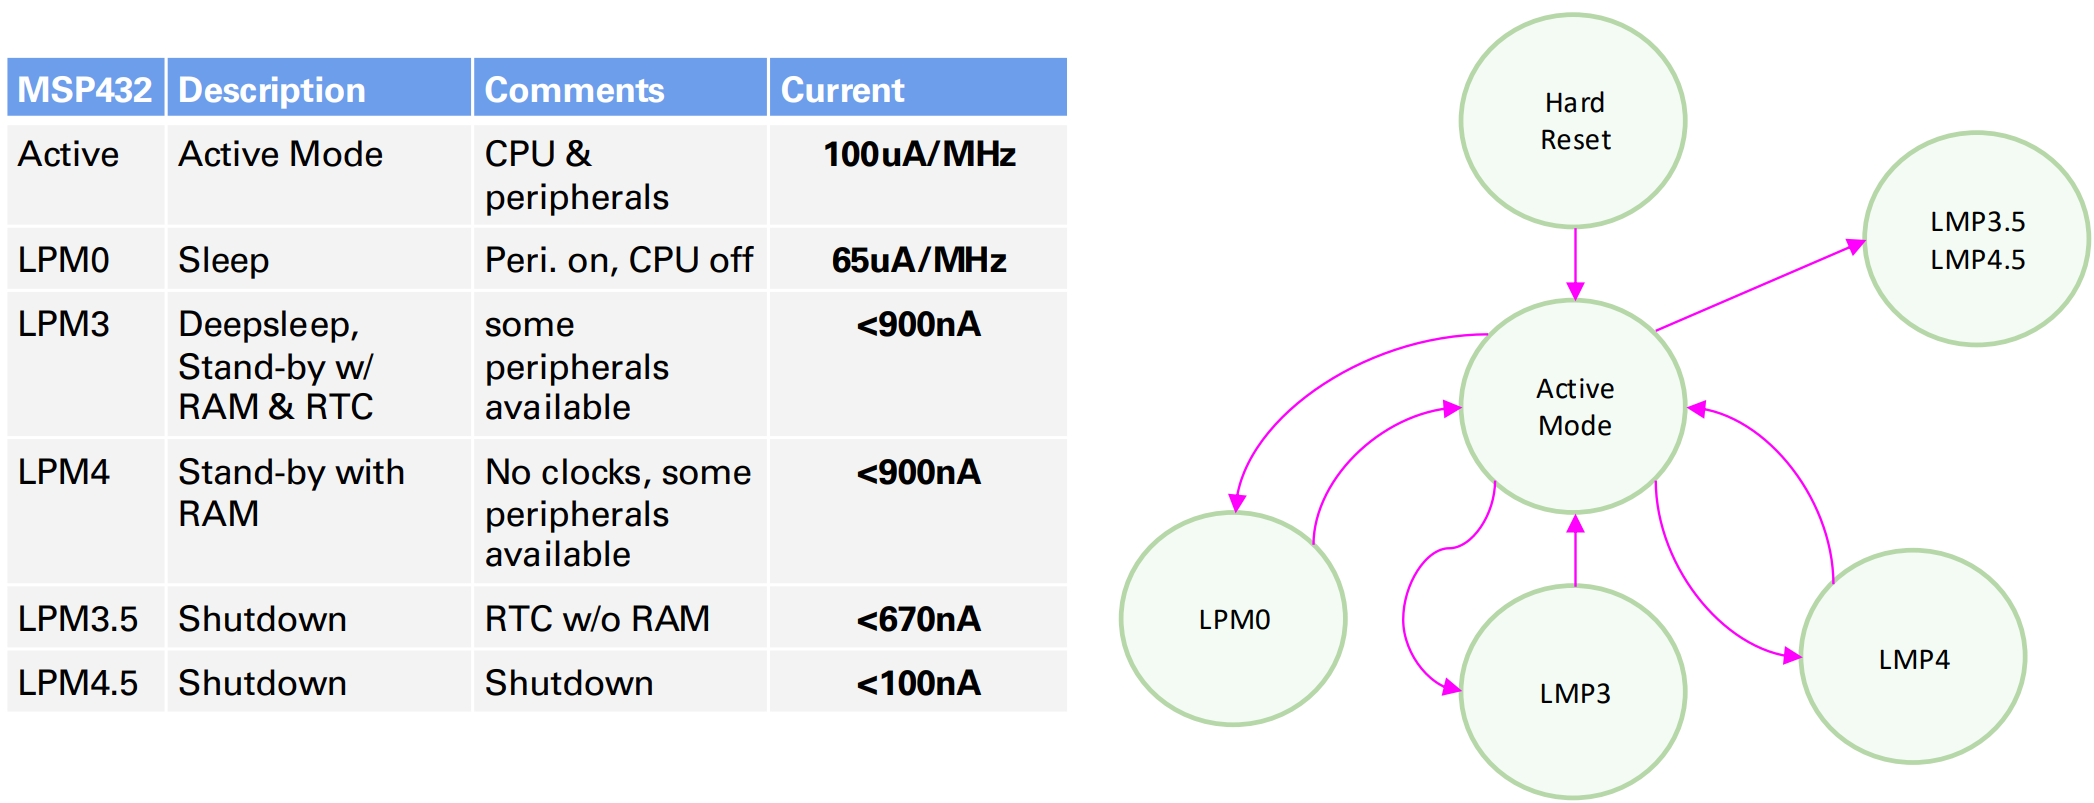
\includegraphics[width=0.9\linewidth]{img/image_63.png}
\end{figure}

To enter LPM0 mode, simply use: \verb|__sleep();|